%!TEX root = causalityRetweetPropensity.tex
\section{Discovering Causal Structure}
As discussed above, our goal is to identify the variables that cause or influence retweet propensity. The variables that we consider in this work are friends count, status count, followers count, klout score and sentiment. As a first step, we try to identify if there is any causal structure involving retweets. We use the PC algorithm described below. 
\subsection{The PC Algorithm}

• For each X and Y, see if X is independent of Y; if so, remove their edge.
• For each X and Y which are still connected, and each third variable Z, see if
X is independent of Y given \{Z\}; if so, remove the edge between X and Y.
• For each X and Y which are still connected, and each third and fourth variables
Z1 and Z2, see if X is independent of Y given \{Z1,Z2\}; if so, remove their edge.

The PC algorithm has two main steps. In the first step, from the data, it learns a skeleton graph, i.e., a graph with only undirected edges. As a second step, it orients the undirected edges to form a markov equivalence class of DAGs. PC algorithm is based on the fact that, if there is no edge between variables A and B, then there is a set of vertices C either connected to A or B such that A is independent of B, conditioned on C, or C d-separates A and B. \\
\begin{center}
\begin{figure}
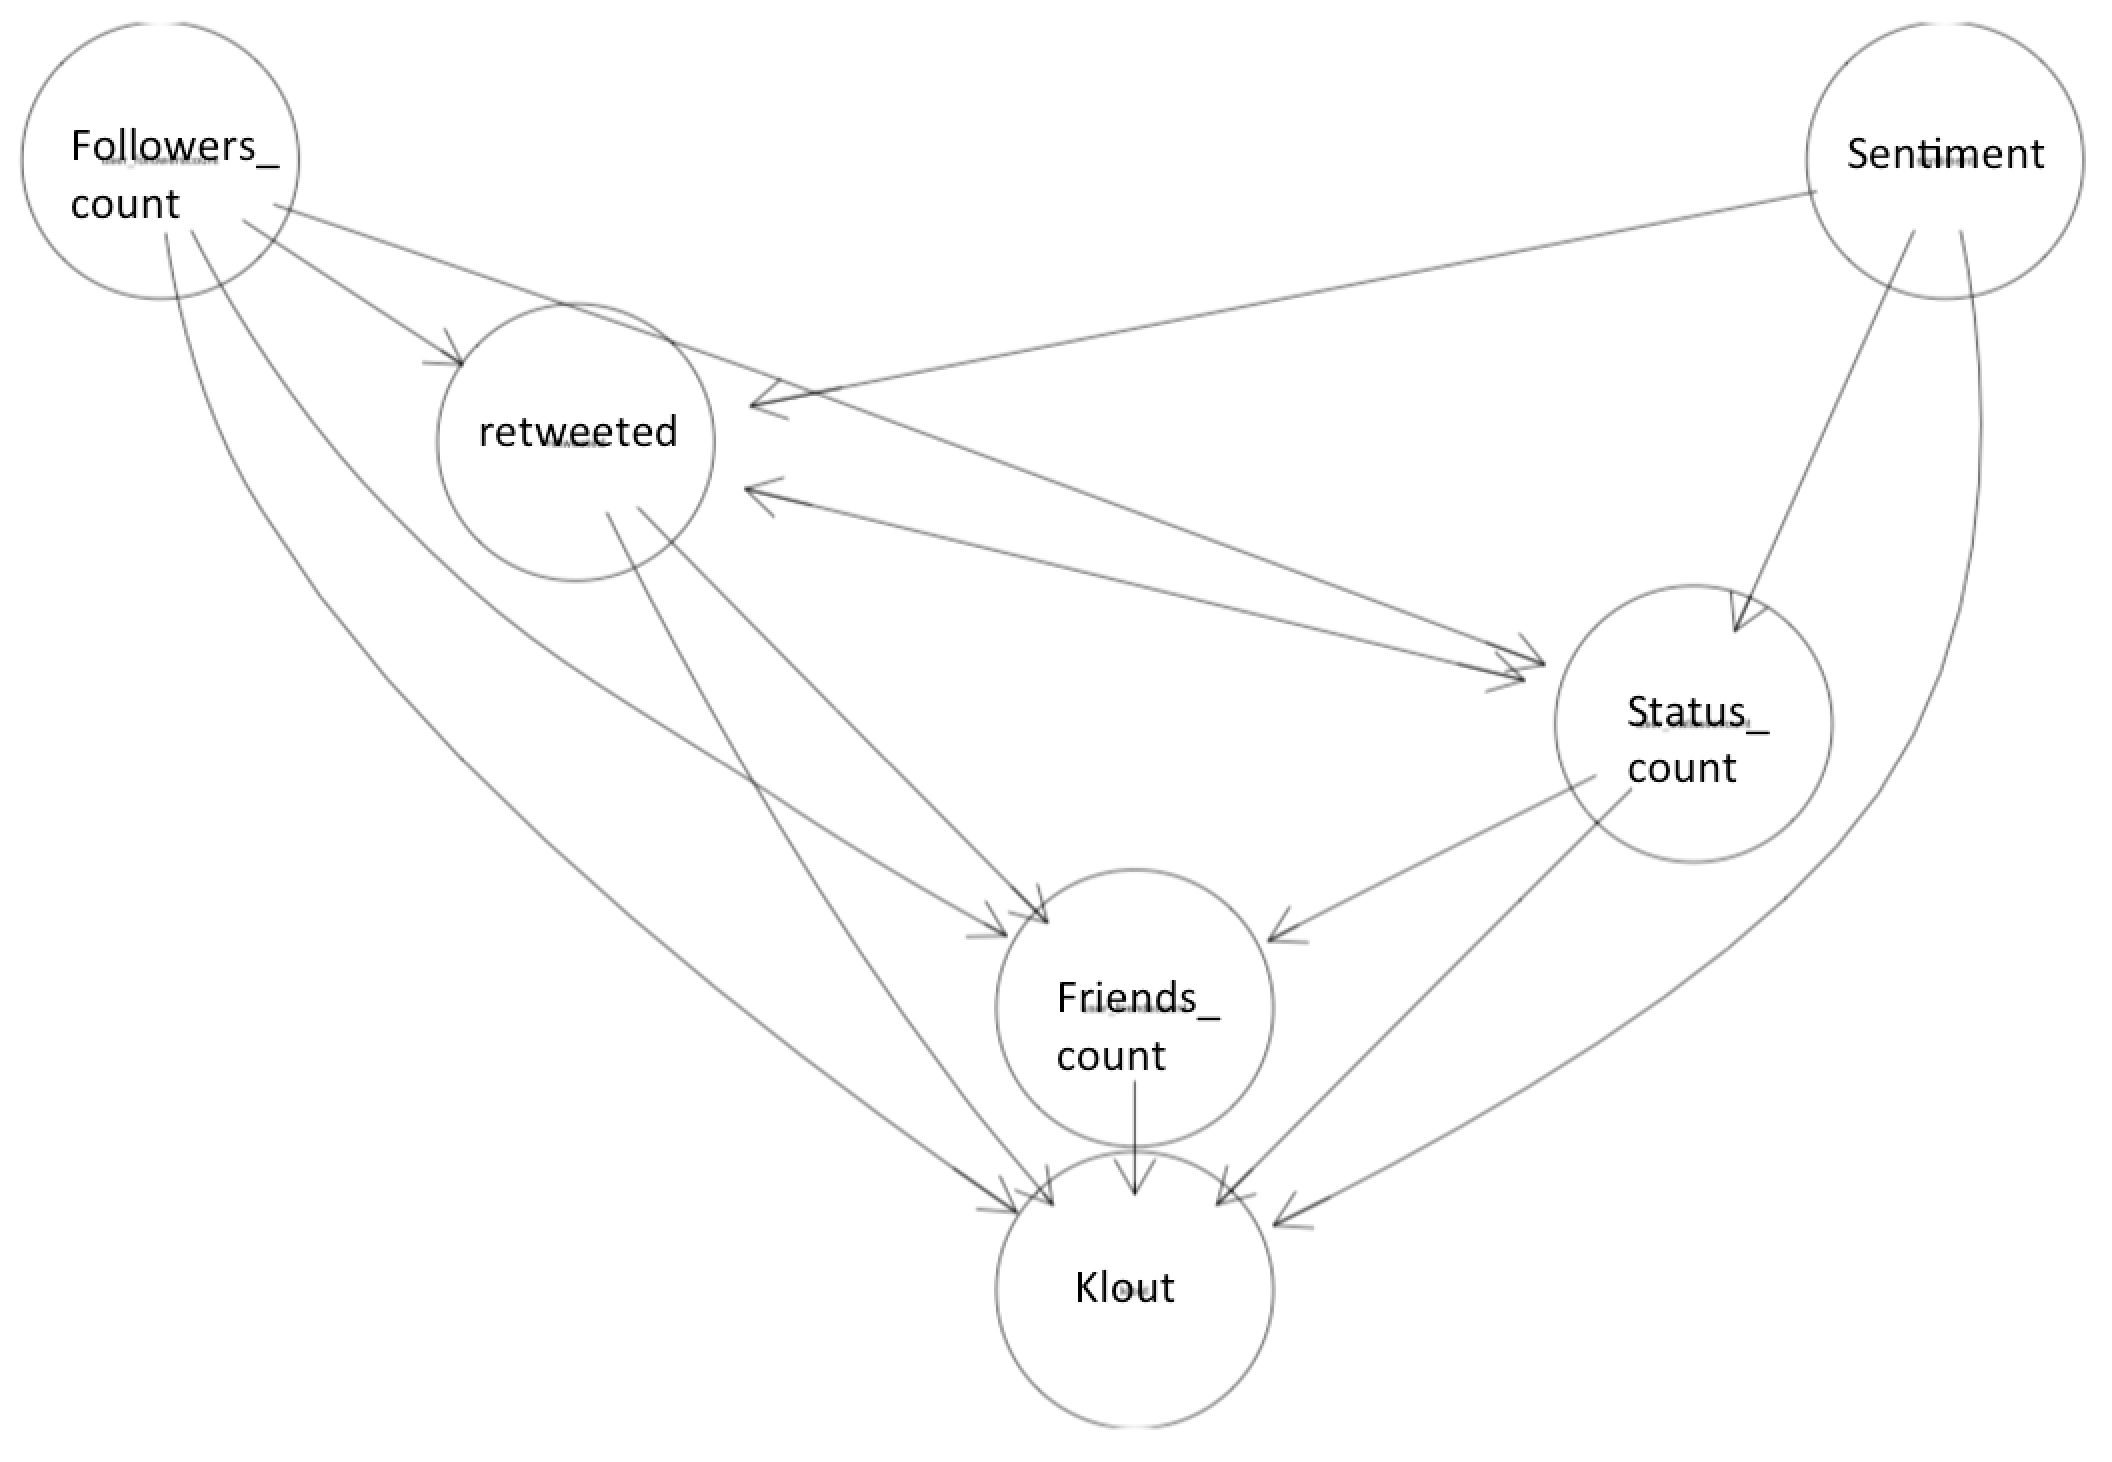
\includegraphics[scale=0.2]{pc}
\end{figure}
\end{center}

